\documentclass[convert={outext=.png}]{standalone}
\usepackage{tikz}

% Compile with: lulatex -shell-escape vrft_block_diagram_standalone.tex

\tikzset{
	block/.style  = {draw, fill=white, rectangle, minimum height=3em, minimum width=5em, node distance = 2cm},
	sum/.style    = {draw, fill=white, circle, node distance=1cm},
	input/.style  = {coordinate},
	output/.style = {coordinate},
	hidden/.style  = {coordinate},
}

\begin{document}
	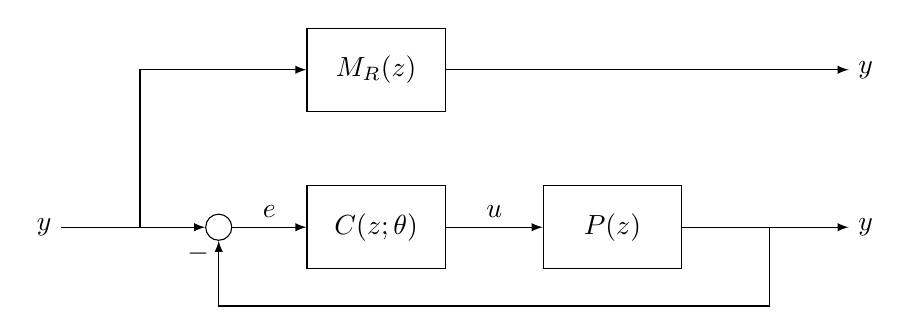
\begin{tikzpicture}[auto, >=latex]
		% Draw the main control loop nodes
		\draw
		node[input] (input) {}
		node[hidden, right of = input     ] (inputfork) {}
		node[sum   , right of = inputfork ] (sum) {}
		node[block , right of = sum       ] (controller) {$C(z; \theta)$}
		node[block , right of = controller, node distance = 3cm] (plant) {$P(z)$}
		node[hidden, right of = plant     , node distance = 2cm] (outputfork) {}
		node[output, right of = outputfork] (output) {}
		node[hidden, below of = plant     ] (retroaction) {};
		
		% Draw the reference model nodes
		\draw
		node[block , above of = controller] (refmodel) {$M_R(z)$}
		node[coordinate, right of = refmodel, node distance = 6cm] (refoutput) {};
		
		% Connect everything together
		\draw[->] node[left] {$y°$} (input) -- (inputfork)  -- (sum);
		\draw[->] (sum) -- (controller) node[midway] {$e$};
		\draw[->] (controller) -- (plant) node[midway] {$u$};
		\draw[->] (plant) -- (outputfork) -- (output) node[right] {$y$};
		
		\draw[->] (outputfork) |- (retroaction) -| node[pos=0.9] {$-$} (sum);
		
		\draw[->] (inputfork) |- (refmodel);
		\draw[->]  (refmodel) -- (refoutput) node[right] {$y$};
	\end{tikzpicture}
\end{document}